\documentclass[14pt]{extarticle}

\let\Overrightarrow\overrightarrow
\let\vecarrow\overrightarrow

%other%
\usepackage{graphicx}
\usepackage{float}
\usepackage[margin=0.7in]{geometry}
\usepackage{caption}
\usepackage{csquotes}
\usepackage[export]{adjustbox}
\usepackage{wrapfig}
\usepackage{setspace}
\usepackage{anyfontsize}
\usepackage{titlesec}
\titleformat{\section}{\normalfont\fontsize{20}{20}\bfseries}{\thesection}{1em}{}
\titleformat{\subsection}{\normalfont\fontsize{17}{20}\bfseries}{\thesubsection}{0.1em}{}
\usepackage{relsize}
\usepackage{indentfirst}
\usepackage{lipsum}
\usepackage{fancybox,framed}
\usepackage{comment}
\usepackage{enumitem}
\usepackage{biolinum}
%other%


%math%
\usepackage[fleqn]{amsmath}
\usepackage{amsthm}
\usepackage{nccmath}
\usepackage{amsmath}
\usepackage{amssymb}
\usepackage{mathtools}
\usepackage{yfonts}
%\usepackage{BOONDOX}

\usepackage{unicode-math}
\setmathfont{Latin Modern Math}

%\usepackage{unicode-math}
%\newtheorem*{}{\textup{Лемма}}
\newtheoremstyle{definition}
{3pt}
{3pt}
{\upshape}
{}
{\itshape\bfseries\fontsize{15}{15}}
{.}
{.5em}
{}
\theoremstyle{definition}
\newtheorem*{definition}{Определение}


%\newtheorem*{theorem}{\normalfont\fontsize{15}{15}\textup{Теорема}}
\newtheoremstyle{theorem}
{3pt}
{3pt}
{\itshape}
{}
{\bfseries\upshape\fontsize{15}{15}}
{.}
{.5em}
{}
%{\thmname{#1}\thmnumber{ #2}\thmnote{ (#3)}}

\usepackage{tikz}
   \usetikzlibrary{calc}

\newcommand{\arc}[0]{
   \tikz [baseline = (N.base), every node/.style={}] {
	  \node [inner sep = 0pt] (N){}; %{$#0$};
      \draw [line width = 0.8pt] plot [smooth, tension=1.3] coordinates {
         ($(N.north west) + (-1.5ex,0.6ex+0.4ex)$)
         ($(N.north)      + (-0.75ex,0+0.4ex)$)
         ($(N.north east) + (0ex,0.6ex+0.4ex)$)
      };
   }
}


\newcommand{\theoremmark} {
\tikz [baseline = (N.base), roundnode/.style={inner sep = 3pt, circle, draw=black!90, 
fill=white, very thick, minimum size=5mm},] {
\node [roundnode] (N){Т}    
    }
}


\theoremstyle{theorem}
\newtheorem*{theorem}{\theoremmark Теорема}

%\newcommand

%\newtheorem*{named}{\innerheader}

\newenvironment{namedtheorem}[2]
{
\newcommand{\foo}{#1}
\newtheorem*{\foo{}}{\normalfont\fontsize{15}{15}{\theoremmark Теорема #2}}
\begin{\foo{}}
}
{\end{\foo{}}}

%\newtheoremstyle{named}{}{}{\itshape}{}{\bfseries}{.}{.5em}{\thmnote{#3's}#1}
%\theoremstyle{named}
%\newtheorem*{namedtheorem}{theorem}
\newtheorem*{remark}{\textup{Комментарий}}
%\renewcommand\qedsymbol{$\blacksquare$}
%\usepackage{parski}
\renewenvironment{proof}
    {\noindent \textit{Доказательство.}\\
	\indent $\square$}
	{ $\blacksquare$\\ }

\newenvironment{solution}
	{\noindent\textbf{Решение.}}


\renewenvironment{remark}
    {\noindent\textbf{Комментарий.}}

\newenvironment{note}
    {\noindent {\normalfont\fontsize{14}{14}\textbf{\textit{Примечание.}}}}



\renewenvironment{rcases}
  {\left.\begin{aligned}}
  {\end{aligned}\right\rbrace}

\DeclarePairedDelimiter\abs{\lvert}{\rvert}
\DeclarePairedDelimiter\norm{\lVert}{\rVert}


%\newcounter{example}[section]
\newenvironment{example}[1]{\noindent \textbf{Пример #1.}}
%\newcommand{\mathleft}{\mathindent0pt}
%{\@fleqntrue}
%\@mathmargin0pt}
%math%

%fonts%
\usepackage[russian]{babel}
\usepackage{polyglossia}
\setdefaultlanguage[spelling=modern]{russian}
%\setotherlanguage{english}
\setmainfont{CMU Serif}
\setsansfont{CMU Sans Serif}
\setmonofont{CMU Typewriter Text}  
%\setmathfont{Latin Modern Math}

%\usepackage{fontspec}

%fonts%


\begin{document}

\begin{figure}[H]
\centering
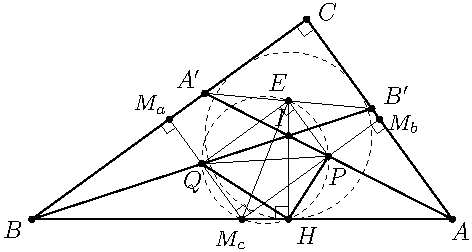
\includegraphics[width=14cm]{./figure.pdf}
\end{figure}

Пусть \(A'\) и \(B'\) --- основания биссектрисс из углов \(A\) и 
\(B\) соответственно; \(M_c\), \(M_b\), \(M_a\) --- середины сторон 
\(AB\), \(AC\), \(BC\) соответственно; \(I\) --- инцентр треугольника 
\(ABC\), а \(E\) --- середина отрезка \(A'B'\). 

Сперва заметим, что \(EQM_cP\) --- прямоугольник. Действительно, он 
параллелограмм, так как \(EP = QM_c = \dfrac{B'A}{2}\) и \(QM_c 
\parallel B'A \parallel EP\), и \(\angle QM_cP = \angle C = 90^{\circ}\)
(\(M_aM_c \parallel CA \perp CB \parallel M_bM_c\)). Таким образом, 
\(QEPM_c\) -- вписанный, причём \(QP\) и \(EM_c\) -- диаметры описанной 
около него окружности. Заметим теперь, что нам осталось показать, что точка 
\(H\) также принадлежит указанной окружности. В самом деле, тогда угол 
\(QHP\) будет прямым, как угол, опирающийся на диаметр \(QP\). 
Для этого необходимо и достаточно доказать, что \(E\), \(I\), \(H\) 
-- коллинеарны. Тогда из условия имеем, что угл \(EHM_c\) -- прямой, а 
значит \(H\) лежит на нашей окружности. \\


\textbf{\textit{Лемма.}} \(E\), \(I\), \(H\) -- коллинеарны.\\
Покажем, что \(IH\) пересекает \(A'B'\) в середине. 
Пусть \(\angle A = 2 \alpha\) и \(\angle B = 2 \beta\), и пусть \(IH \cap 
A'B' = F\). Далее, \(\angle A'IE = \angle AIH = 90^{\circ} - \alpha\), 
\(\angle B'IE = \angle BIH = 90^{\circ} - \beta\). 

Покажем, что \(S_{IFA'} = S_{IFB'}\), что и будет означать, что \(F = E\).
Мы знаем, что \(S_{IFA'} = \dfrac{IF \cdot IA' \cdot \sin{(90^{\circ} - 
\alpha)}}{2}\)
и что \(S_{IFB'} = \dfrac{IF \cdot IB' \cdot \sin{(90^{\circ} - 
\beta)}}{2}\). То есть осталось показать, что \(IA' \cdot \cos{\alpha} = 
IB' \cdot \cos{\beta}\). Остаётся заметить, что \(IA' \cdot \cos{\alpha} = 
r = IB' \cdot \cos{\beta}\), где \(r\) -- радиус вписанной в \(ABC\) 
окружности.


\end{document}
